\documentclass[12pt,a4paper,UTF8]{ctexart}
\usepackage{graphicx}
\usepackage{amsmath}
\usepackage{amssymb}
\usepackage{cite}
\usepackage[ntheorem]{empheq}
\usepackage{enumitem}
\usepackage{fullpage}
\usepackage{tocbibind}
\usepackage[bookmarksopen=true,colorlinks,linkcolor=black]{hyperref}
\usepackage{cellspace}
\usepackage{listings}
\usepackage{color}
\usepackage{epstopdf}
\usepackage{subfigure}
\usepackage{algorithm}
\usepackage{algorithmicx}
\usepackage{algpseudocode}
\usepackage{lipsum}
\usepackage[thmmarks,amsmath]{ntheorem}



\theoremstyle{nonumberplain}

\theoremheaderfont{\bfseries}

\theorembodyfont{\normalfont}

\theoremsymbol{$\square$}

\newtheorem{Proof}{\hskip 2em 证明}


\makeatletter
\newenvironment{breakablealgorithm}
  {% \begin{breakablealgorithm}
   \begin{center}
     \refstepcounter{algorithm}% New algorithm
     \hrule height.8pt depth0pt \kern2pt% \@fs@pre for \@fs@ruled
     \renewcommand{\caption}[2][\relax]{% Make a new \caption
       {\raggedright\textbf{\ALG@name~\thealgorithm} ##2\par}%
       \ifx\relax##1\relax % #1 is \relax
         \addcontentsline{loa}{algorithm}{\protect\numberline{\thealgorithm}##2}%
       \else % #1 is not \relax
         \addcontentsline{loa}{algorithm}{\protect\numberline{\thealgorithm}##1}%
       \fi
       \kern2pt\hrule\kern2pt
     }
  }{% \end{breakablealgorithm}
     \kern2pt\hrule\relax% \@fs@post for \@fs@ruled
   \end{center}
  }
\makeatother
\renewcommand{\algorithmicrequire}{\textbf{Input:}}  % Use Input in the format of Algorithm
\renewcommand{\algorithmicensure}{\textbf{Output:}} % Use Output in the format of Algorithm
\usepackage{longtable}

\usepackage{float}
\definecolor{gray}{rgb}{0.5,0.5,0.5}
\definecolor{dkgreen}{rgb}{.068,.578,.068}
\definecolor{dkpurple}{rgb}{.320,.064,.680}

% set Matlab styles
\lstset{
   language=Matlab,
   numbers=left,
   keywords={break,case,catch,continue,else,elseif,end,for,function,
      global,if,otherwise,persistent,return,switch,try,while},
   basicstyle=\ttfamily,
   keywordstyle=\color{blue}\bfseries,
   commentstyle=\color{dkgreen},
   stringstyle=\color{dkpurple},
   backgroundcolor=\color{white},
   breaklines=true,
   tabsize=4,
   showspaces=false,
   showstringspaces=false,
}

\begin{document}
\CJKfamily{zhkai}


\begin{center}
    \textbf{作业二}\\
    \textbf{姓名 胡毅翔 ~~ 学号 PB18000290 ~~ 日期 2021年5月29日}\\
\end{center}

\begin{center}
    \fbox{
        \begin{minipage}{40em}
            \vspace{5cm}
            \hspace{20cm}
        \end{minipage}}
\end{center}
\vspace{1cm}

\begin{enumerate}
    \item[第一题] 本题考虑使用Richardson外推技术提高向前差商求给定函数导数的精度。
          \begin{enumerate}\item  (5分)使用向前差分计算 $f(x)=\sin (x)$ 在 $x=1.2$ 处的导数并使用loglog图 展示其精度随离散区间大小 $h$ 的变化。 $h$ 取 $10^{0}, 10^{-1}, 10^{-2}, 10^{-3}, \ldots, 10^{-15}$ 。
                    \par 解:
                    \par 本题的\textbf{MATLAB}程序显示如下:
                    \begin{lstlisting}[frame=single]
clear,clc

syms x;
F = @(x) sin(x);
result = [0:15];
h_l = result;
tmp = cos(1.2);
f = F(1.2);

for i = 0:15
    h = 10^(-i);
    h_l(i + 1) = h;
    result(i + 1) = abs((F(1.2 + h) - f) / h - tmp);
end

loglog(h_l, result);
\end{lstlisting}
                    \par 程序运行输出结果为:
                    \begin{figure}[H]
                        \centering
                        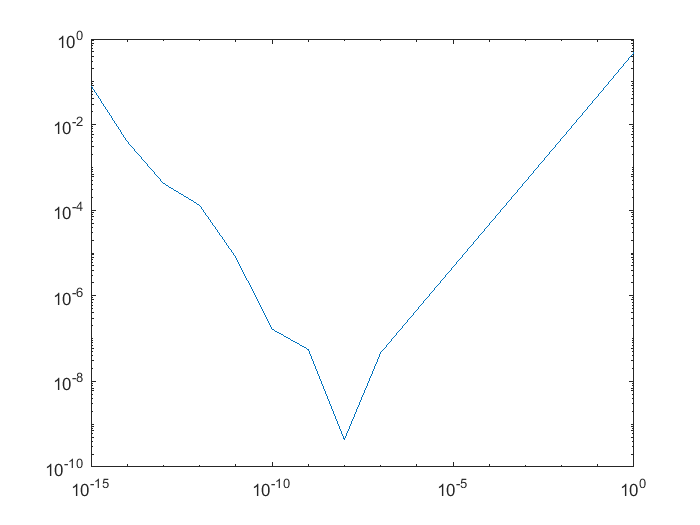
\includegraphics[scale=0.45]{1_1.png}
                        \caption{向前差分精度随离散区间大小h的变化的情况}
                    \end{figure}
              \item(10分)推导出使用Richardson外推技术的向前差商的计算公式并用伪代码 给出算法。
                    \par 解:
                    $$
                        f\left(x_{0}+h\right)=f\left(x_{0}\right)+h f^{\prime}\left(x_{0}\right)+\frac{h^{2}}{2 !} f^{\prime \prime}\left(x_{0}\right)+\frac{h^{3}}{3 !} f^{\prime \prime \prime}\left(x_{0}\right)+\frac{h^{4}}{4 !} f^{(4)}\left(x_{0}\right)+O\left(h^{5}\right) \\
                        ((2)-(1)) / 2
                    $$
                    得
                    $$f^{\prime}\left(x_{0}\right)=\frac{1}{ h}\left[f\left(x_{0}+h\right)-f\left(x_{0}\right)\right]+\frac{h}{2} f^{(2)}\left(x_{0}\right)+O\left(h^{3}\right)
                    $$
                    记
                    $$N_{1}(h)=\frac{f\left(x_{0}+h\right)-f\left(x_{0}\right)}{ h} $$
                    $$f^{\prime}\left(x_{0}\right)=N_{1}(h)+\frac{h}{2} f^{(2)}\left(x_{0}\right)+O\left(h^{2}\right) $$

                    $$f^{\prime}\left(x_{0}\right)=N_{1}\left(\frac{h}{2}\right)+\frac{1}{2}\left(\frac{h}{2}\right) f^{(2)}\left(x_{0}\right)+O\left(h^{2}\right)$$
                    $$f^{\prime}\left(x_{0}\right)=\frac{1}{2-1}\left(2 N_{1}\left(\frac{h}{2}\right)-N_{1}(h)\right)+O\left(h^{2}\right) \approx N_{2}(h) $$
                    $$N_{2}(h)=N_{1}\left(\frac{h}{2}\right)+\frac{N_{1}\left(\frac{h}{2}\right)-N_{1}(h)}{2-1}
                    $$
                    继续外推下去, 得到
                    $$N_{j}(h)=N_{j-1}\left(\frac{h}{2}\right)+\frac{N_{j-1}\left(\frac{h}{2}\right)-N_{j-1}(h)}{2^{j-1}-1}, \quad j=2,3, \cdots
                    $$
                    伪代码如下:
                    \begin{breakablealgorithm}
                        \caption{Forward Difference Quotient with Richardson Extrapolation}
                        \label{alg::conjugateGradien}
                        \begin{algorithmic}[1]
                            \Require
                            $h$:initial value of h;

                            $maxrept$: the maximum number of iterations;

                            $\varepsilon $: error size;

                            \Ensure
                            $f^{\prime}\left(x_{0}\right)$: the estimated value which is closest to $f^{\prime}\left(x_{0}\right)$;

                            $error message$: if the input cannot be resolved by algorithm;
                            \State $A.length$ $\leftarrow$ $2$;
                            \State $A\left[1\right]$ $\leftarrow$ $N_{1}\left(h\right)$;
                            \State $A\left[2\right]$ $\leftarrow$ $N_{1}\left(\frac{h}{2}\right)$;
                            \State $tmp$ $\leftarrow$ $2A\left[2\right]-A\left[1\right]$;
                            \While {$\left\lvert tmp-A\left[1\right]\right\rvert \geq \varepsilon  \ and\ A.length \leq maxrept $}
                            \State $A\left[1\right]$ $\leftarrow$ $tmp$;
                            \State $A.length$ $\leftarrow$ $A.length + 1$;
                            \State $A\left[A.length\right]$ $\leftarrow$ $N_{1}\left(\frac{h}{2^{A.length-1}}\right)$;
                            \For {$i$ = $1$ \textbf{to} $A.length - 2$ }
                            \State $A\left[A.length-i\right]$ $\leftarrow$ $A\left[A.length-i+1\right]+\frac{A\left[A.length-i+1\right]-A\left[A.length-i\right]}{2^{i}-1}$;
                            \EndFor
                            \State $tmp$ $\leftarrow$ $A\left[2\right]+\frac{A\left[2\right]-A\left[1\right]}{2^{A.length-1}-1}$;
                            \EndWhile
                            \If{$A.length > maxrept$}
                            \State \textbf{error message};
                            \Else
                            \State \textbf{return} $tmp$;
                            \EndIf
                        \end{algorithmic}
                    \end{breakablealgorithm}
              \item(5分)使用你的算法计算 $f(x)=\sin (x)$ 在 $x=1.2$ 处的导数并使用semilogy图 展示其精度随外推次数变化的情况。请自己选取h初始值,使得用外推方法
                    能够算出的最精确的导数尽量精确。你的回答需要说明你使用外推方法算出
                    的导数值是多少、误差又是多少、h的初始值是多少、外推了多少次。
                    \par 解:
                    \par 本题的\textbf{MATLAB}程序显示如下:
                    \begin{lstlisting}[frame=single]
clear,clc,close all

syms x;
F = @(x)sin(x);
maxrept = 50;
a = cos(1.2);

for i = 0:15
    h = 10^(-i);

    for k = -15:-5
        epslion = 10^(k);
        A(1) = N(h);
        A(2) = N(h / 2);
        tmp = 2 * A(2) - A(1);

        if i == 0
            B(1) = abs(N(h) - a);
            B(2) = abs(tmp - a);
        end

        while abs(tmp - A(1)) >= epslion && length(A) <= maxrept

            A(1) = tmp;
            A(length(A) + 1) = N(h / (2^(length(A) - 1)));

            for j = 1:length(A) - 2
                A(length(A) - j) = A(length(A) - j + 1) + (A(length(A) - j + 1) - A(length(A) - j)) / (2^j - 1);
            end

            tmp = A(2) + (A(2) - A(1)) / (2^(length(A) - 1) - 1);

            if i == 0
                B(length(A)) = abs(tmp - a);
            end

        end

        if length(A) <= maxrept && abs(tmp) > epslion
            X = sprintf('h:10^%d tmp:%.15f epslion:10^%d n:%d delta:%.15f', -i, tmp, k, length(A), abs(tmp - a));
            disp(X)
            break;
        end

        if i == 0
            B = [];
        end

        A = [];
    end

end

semilogy(1:length(B), B);

function result = N(h)
    syms y;
    F = @(y)sin(y);
    result = (F(1.2 + h) - F(1.2)) / h;
end
\end{lstlisting}
                    \par 程序运行的输出结果为:
                    \begin{lstlisting}[frame=single]
h:10^0 tmp:0.362357754476664 epslion:10^-13 n:12 delta:0.000000000000010
h:10^-1 tmp:0.362357754478041 epslion:10^-11 n:11 delta:0.000000000001367
h:10^-2 tmp:0.362357754474414 epslion:10^-11 n:11 delta:0.000000000002260
h:10^-3 tmp:0.362357754498787 epslion:10^-10 n:10 delta:0.000000000022113
h:10^-4 tmp:0.370652071522364 epslion:10^-11 n:34 delta:0.008294317045690
h:10^-5 tmp:0.362357755880015 epslion:10^-8 n:8 delta:0.000000001403341
h:10^-6 tmp:0.362357759856709 epslion:10^-8 n:7 delta:0.000000005380035
h:10^-7 tmp:0.362357752692333 epslion:10^-7 n:2 delta:0.000000001784341
h:10^-8 tmp:0.362357777117239 epslion:10^-7 n:2 delta:0.000000022640566
h:10^-9 tmp:0.362358032468535 epslion:10^-6 n:2 delta:0.000000277991861
h:10^-10 tmp:0.362359031782951 epslion:10^-8 n:6 delta:0.000001277306278
h:10^-11 tmp:0.362376795219604 epslion:10^-8 n:7 delta:0.000019040742931
h:10^-12 tmp:0.362376783868240 epslion:10^-6 n:6 delta:0.000019029391566
h:10^-15 tmp:0.444089209850063 epslion:10^-15 n:2 delta:0.081731455373389  
\end{lstlisting}
                    \par 其中$h$为初始值,
                    $tmp$为算出的导数值,$epslion$为设置的误差限,$n$为外推次数,$delta$为计算的结果与\textbf{MATLAB}计算的在$x=1.2$处的导数值$cos(1.2)$的差值。
                    \par 故选取$h$初始值为$10^0$,算出的导数值为$0.362357754476664$,误差为$0.000000000000010$,外推了$12$次,得到的semilogy图为:
                    \begin{figure}[H]
                        \centering
                        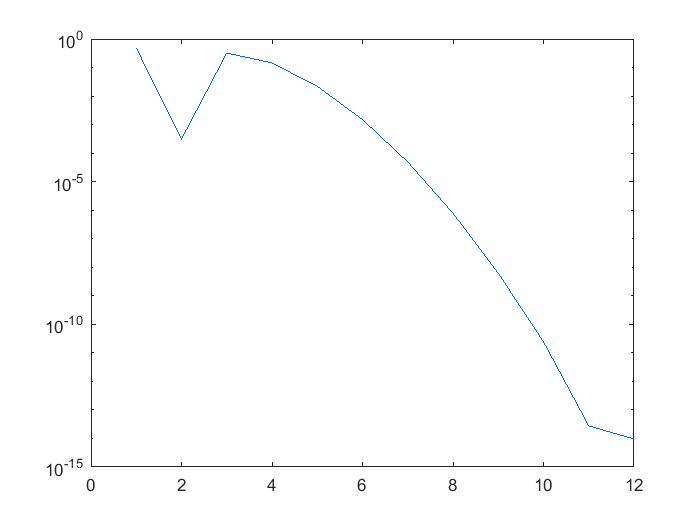
\includegraphics[scale=0.45]{1_3.png}
                        \caption{精度随外推次数变化情况(h=0)}
                    \end{figure}
          \end{enumerate}
    \item[第二题] 本题讨论使用复化梯形公式求周期函数的积分。
          \begin{enumerate}
              \item
                    (10分)证明当 $r$ 不是 $m$ 的整倍数的情况下,使用 $m$ 个子区间的复化梯形公式
                    可以精确积分
                    $$
                        \int_{-\pi}^{\pi} \cos (r x) d x  \text { 和 }  \int_{-\pi}^{\pi} \sin (r x) d x
                    $$
                    注意:这一结论类似于课堂上我们定义的代数精度。同时说明如果 $r$ 为 $m$ 的
                    整倍数时复化梯形公式对于上面两个积分会给出怎样的结果。
                    \par 解:
                    \par
                    $$
                        T(h)=T_{n}(f)=h\left[\frac{1}{2} f(a)+\sum_{i=1}^{n-1} f(a+i h)+\frac{1}{2} f(b)\right]
                    $$
                    $$\begin{aligned}
                            T\left(\frac{2\pi}{m}\right)= & \frac{2\pi}{m}\left[\frac{1}{2} f(-\pi)+\sum_{i=1}^{m-1} f(-\pi+i \frac{2\pi}{m})+\frac{1}{2} f(\pi)\right]            \\
                            =                             & \frac{2\pi}{m}\left[\frac{1}{2} cos(-r\pi)+\sum_{i=1}^{m-1} cos(r(-\pi+i \frac{2\pi}{m}))+\frac{1}{2} cos(r\pi)\right] \\
                            =                             & \frac{2\pi}{m}sin(r\pi)\left(cos\left(r\pi\right)cot\left(\frac{r\pi}{m}\right)+sin(r\pi)\right)\end{aligned}
                    $$
                    则$r$为$m$的整数倍$(r=km)$时
                    $$T(h)={2\pi}cos(r\pi)$$
                    若$r$不是$m$的整数倍
                    $$T(h)=0$$
                    同理当$f(x)=sin(rx)$时,
                    $$T\left(\frac{2\pi}{m}\right)=\frac{\pi}{m}\left(cos\left(\frac{r\pi}{m}\right)-cos\left(\frac{r\pi (2m-1)}{m}\right)\right)csc(\frac{r\pi}{m})=0$$

              \item (10分)由于任意的以 $2 \pi$ 为周期的周期函数都可以表示为由正弦与余弦函数 的线性组合,所以上一问中所证明的定理实际上告诉我们求解一个周期函 数的积分的有效方法正是复化梯形公式。现使用复化梯形公式和不同数量 的子区间个数来求 $f(x)=e^{\cos (x)}$ 在 $[-\pi, \pi]$ 的积分,并用这个函数的真实积分 值作为参照使用semilogy图画出随着子区间数量 $m$ 变化所得到的积分精度 的变化。
                    \par 题后语: 复化梯形公式之于周期函数的积分如同Gauss积分公式之于非周期
                    函数的基于多项式的积分。因此复化梯形公式是最有效的求解周期函数积分 的方法。
                    \par 解:
                    $$\int_{-\pi}^{\pi} e^{cos(x)} dx =  2\pi I_0(1)\approx 7.95492652101284527451$$
                    \par 本题的\textbf{MATLAB}程序显示如下:
                    \begin{lstlisting}[frame=single]
clc, clear, close all
syms x;
F = @(x) exp(cos(x));
maxrept = 50;
r = 7.95492652101284527451;

for i = 2:maxrept
    h = 2 * pi / i;
    S = F(-pi) / 2 + F(pi) / 2;

    for j = 1:i - 1
        S = S + F(-pi + j * h);
    end

    S = S * h;
    T(i - 1) = abs(S - r);
end

semilogy([2:maxrept], T);
\end{lstlisting}
                    \par 程序运行的输出结果为:
                    \begin{figure}[H]
                        \centering
                        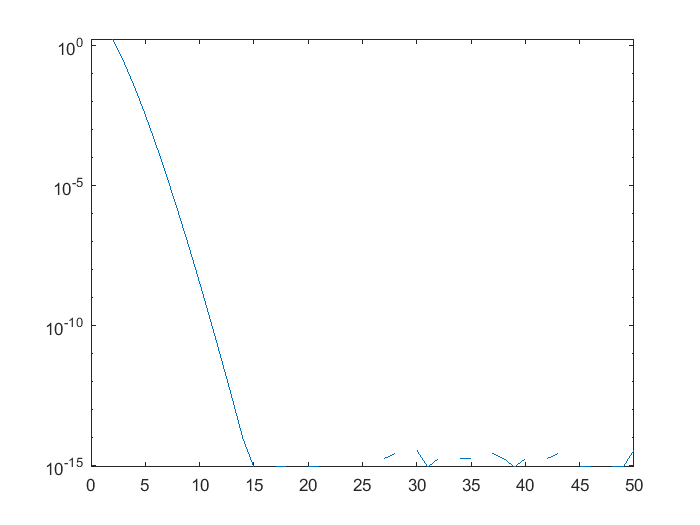
\includegraphics[scale=0.45]{2_2.png}
                        \caption{积分精度随子区间数$m$变化情况}
                    \end{figure}
                    \par 其中未显示的点,表示在机器精度限制下差值为0。
          \end{enumerate}
    \item[第三题]
          \begin{enumerate}
              \item (10分)推导出如下格式的多步法公式:
                    \begin{equation}\label{1}
                        y_{n+1}=y_{n-1}+\alpha f_{n+1}+\beta f_{n}+\gamma f_{n-1}
                    \end{equation}
              \item (10分)推导此格式的局部截断误差,并由此指明此格式的阶数。
                    \par 解:
                    \par 线性多步法的一般形式为$$
                        y_{k+1}=\sum_{i=0}^{r} \alpha_{i} y_{k-i}+h \sum_{i=-1}^{r} \beta_{i} y_{k-i}^{\prime}=\sum_{i=0}^{r} \alpha_{i} y_{k-i}+h \sum_{i=-1}^{r} \beta_{i} f_{k-i}
                    $$
                    局部截断误差为
                    $$
                        R_{k+1}=y\left(x_{k+1}\right)-\left[\sum_{i=0}^{r} \alpha_{i} y_{k-i}+h \sum_{i=-1}^{r} \beta_{i} f_{k-i}\right]
                    $$
                    又有
                    $$
                        \begin{aligned}
                            R_{k+1}= & \left(1-\sum_{i=0}^{r} \alpha_{i}\right) y\left(x_{k}\right)+\sum_{j=1}^{p} \frac{h^{j}}{j !}\left\{1-\left[\sum_{i=1}^{r}(-i)^{j} \alpha_{i}+j \sum_{i=-1}^{r}(-i)^{j-1} \beta_{i}\right]\right\} y^{(j)}\left(x_{k}\right) \\
                                     & +\frac{h^{p+1}}{(p+1) !}\left\{1-\left[\sum_{i=1}^{r}(-i)^{p+1} \alpha_{i}+(p+1) \sum_{i=-1}^{r}(-i)^{p} \beta_{i}\right]\right\} y^{(p+1)}\left(x_{k}\right)+O\left(h^{p+2}\right)
                        \end{aligned}
                    $$
                    要使上式中 $y\left(x_{k}\right), h, h^{2}, \cdots, h^{p}$ 的系数为零, $\alpha_{i}, \beta_{i}$ 就必须满足
                    \begin{equation}\label{33}
                        \left\{\begin{array}{l}
                            \sum_{i=0}^{r} \alpha_{i}=1 \\
                            \sum_{i=1}^{r}(-i)^{j} \alpha_{i}+j \sum_{i=-1}^{r}(-i)^{j-1} \beta_{i}=1, \quad j=0,1,2, \cdots, p
                        \end{array}\right.
                    \end{equation}

                    这是一个含 $2 r+3$ 个待定参数、 $p+1$ 个方程的线性方程组. 此时, 所获得的线性多步法的局 部截断误差为
                    $$
                        R_{k+1}=\frac{h^{p+1}}{(p+1) !}\left\{1-\left[\sum_{i=1}^{r}(-i)^{p+1} \alpha_{i}+(p+1) \sum_{i=-1}^{r}(-i)^{p} \beta_{i}\right]\right\} y^{(p+1)}\left(x_{k}\right)+O\left(h^{p+2}\right)
                    $$
                    如取 $r=1, p=4$, 则由式\ref{33}可得
                    $$
                        \left\{\begin{array}{l}
                            \alpha_{0}+\alpha_{1}=1                      \\
                            -\alpha_{1}+\beta_{-1}+\beta_{0}+\beta_{1}=1 \\
                            \alpha_{1}+2 \beta_{-1}-2 \beta_{1}=1        \\
                            -\alpha_{1}+3 \beta_{-1}+3 \beta_{1}=1       \\
                            \alpha_{1}+4 \beta_{-1}-4 \beta_{1}=1
                        \end{array}\right.
                    $$
                    若取 $\alpha_{0}=0, \alpha_{1}=1, \beta_{-1}=\beta_{1}=1 / 3, \beta_{0}=4 / 3$, 则可得公式
                    $$
                        y_{k+1}=y_{k-1}+h\left(f_{k+1}+4 f_{k}+f_{k-1}\right) / 3
                    $$
                    上式  也称为 Simpson 公式, 其局部截断误差为
                    $$
                        R_{k+1}=\frac{1}{90} h^{5} y_{k}^{(5)}+O\left(h^{6}\right)
                    $$
                    故Simpson公式为二步四阶公式。
              \item (10分)选取合适的步长值,用此格式在 $[0,2]$ 上解如下的初值问题:
                    \begin{equation}\label{2}
                        y^{\prime}=x e^{-4 x}-4 y, \quad y(0)=0
                    \end{equation}

                    使用你刚刚推导出的格式\ref{1},并利用二阶Runge-Kutta方法(即课本公式(7.15))起 步。画出解函数。
                    \par 解:
                    \par 二阶Runge-Kutta方法:
                    $$
                        \left\{\begin{array}{l}
                            y_{n+1}=y_{n}+h k_{2}            \\
                            k_{1}=f\left(x_{n}, y_{n}\right) \\
                            k_{2}=f\left(x_{n}+\frac{h}{2}, y_{n}+\frac{h}{2} k_{1}\right)
                        \end{array}\right.
                    $$
                    预估校正公式:
                    $$
\left\{\begin{array}{l}
\bar{y}_{n+1}=y_{n-1}+\frac{h}{3}\left[7 f\left(x_{n}, y_{n}\right)-2 f\left(x_{n-1}, y_{n-1}\right)+f\left(x_{n-2}, y_{n-2}\right)\right] \\
y_{n+1}=y_{n-1}+\frac{h}{3}\left[3 f\left(x_{n+1}, \bar{y}_{n+1}\right)+4f\left(x_{n}, y_{n}\right)+ f\left(x_{n-1}, y_{n-1}\right)\right]
\end{array}\right.
$$
                    \par 本题的\textbf{MATLAB}程序显示如下:
                    \begin{lstlisting}[frame=single]
clc, clear, close all

syms x;
syms y;
F = @(x, y)x * exp(-4 * x) - 4 * y;
Y_0 = 0;
n = 10^5;
t = 0;
h = 2 / n;
result(1) = Y_0;
k1 = F(t, result(1));
k2 = F(t + h / 2, result(1) + k1 * h / 2);
result(2) = result(1) + k2 * h;
k1 = F(t + h, result(2));
k2 = F(t + h + h / 2, result(2) + k1 * h / 2);
result(3) = result(2) + k2 * h;

for i = 3:n
    tmp = result(i - 1) + h / 3 * (F(t, result(i - 2)) - 2 * F(t + h, result(i - 1)) + 7 * F(t + 2 * h, result(i)));
    result(i + 1) = result(i - 1) + h / 3 * (F(t + h, result(i - 1)) + 4 * F(t + 2 * h, result(i)) + F(t + 3 * h, tmp));
    t = t + h;
end

plot([0:2 / n:2], result);                       
\end{lstlisting}
                    \par 程序运行的输出结果为:
                    \begin{figure}[H]
                        \centering
                        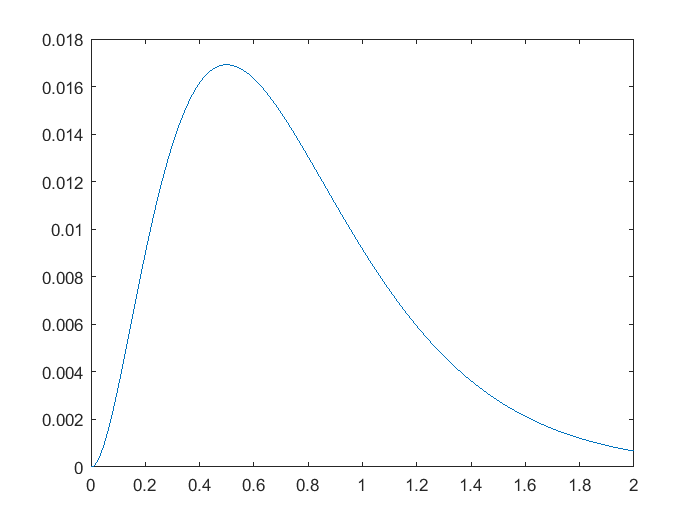
\includegraphics[scale=0.45]{3_3.png}
                        \caption{解函数图像(步长$h=\frac{2}{10^5}$)}
                    \end{figure}
              \item (10分)推导出 \ref{2}的精确解。对比该精确解在 $x=2$ 这一点的值,用log-log图 展示所用方法的阶数,并给出解释。
                    \par 解:
                    $$f(x)=x^2e^{(-4x)}$$
                    $$f^{\prime}(x)=x^2e^{(-4x)}$$
                    故精确解为
                    $$y=\frac{1}{2}x^{2}e^{(-4x)}$$
                    \par 本题的\textbf{MATLAB}程序显示如下:
                    \begin{lstlisting}[frame=single]
clc, clear, close all

syms x;
syms y;
F = @(x, y)x * exp(-4 * x) - 4 * y;
G = @(x)1/2 * x^2 * exp(-4 * x);
Y_0 = 0;

for j = 2:100000
    n = j;
    t = 0;
    h = 2 / n;
    result(1) = Y_0;
    k1 = F(t, result(1));
    k2 = F(t + h / 2, result(1) + k1 * h / 2);
    result(2) = result(1) + k2 * h;
    k1 = F(t + h, result(2));
    k2 = F(t + h + h / 2, result(2) + k1 * h / 2);
    result(3) = result(2) + k2 * h;

    for i = 3:n
        tmp = result(i - 1) + h / 3 * (F(t, result(i - 2)) - 2 * F(t + h, result(i - 1)) + 7 * F(t + 2 * h, result(i)));
        result(i + 1) = result(i - 1) + h / 3 * (F(t + h, result(i - 1)) + 4 * F(t + 2 * h, result(i)) + F(t + 3 * h, tmp));
        t = t + h;
    end

    delta(j - 1) = abs(G(2) - result(n + 1));
    L(j - 1) = h;
end

figure;
subplot(1, 2, 1)
loglog(L, delta);
logl = log10(L);
logd = log10(delta);
t = polyfit(logl, logd, 1);
subplot(1, 2, 2);
plot(logl, logd, '*', logl, polyval(t, logl));                     
\end{lstlisting}
                    \par 程序运行的输出结果为:
                    \begin{figure}[H]
                        \centering
                        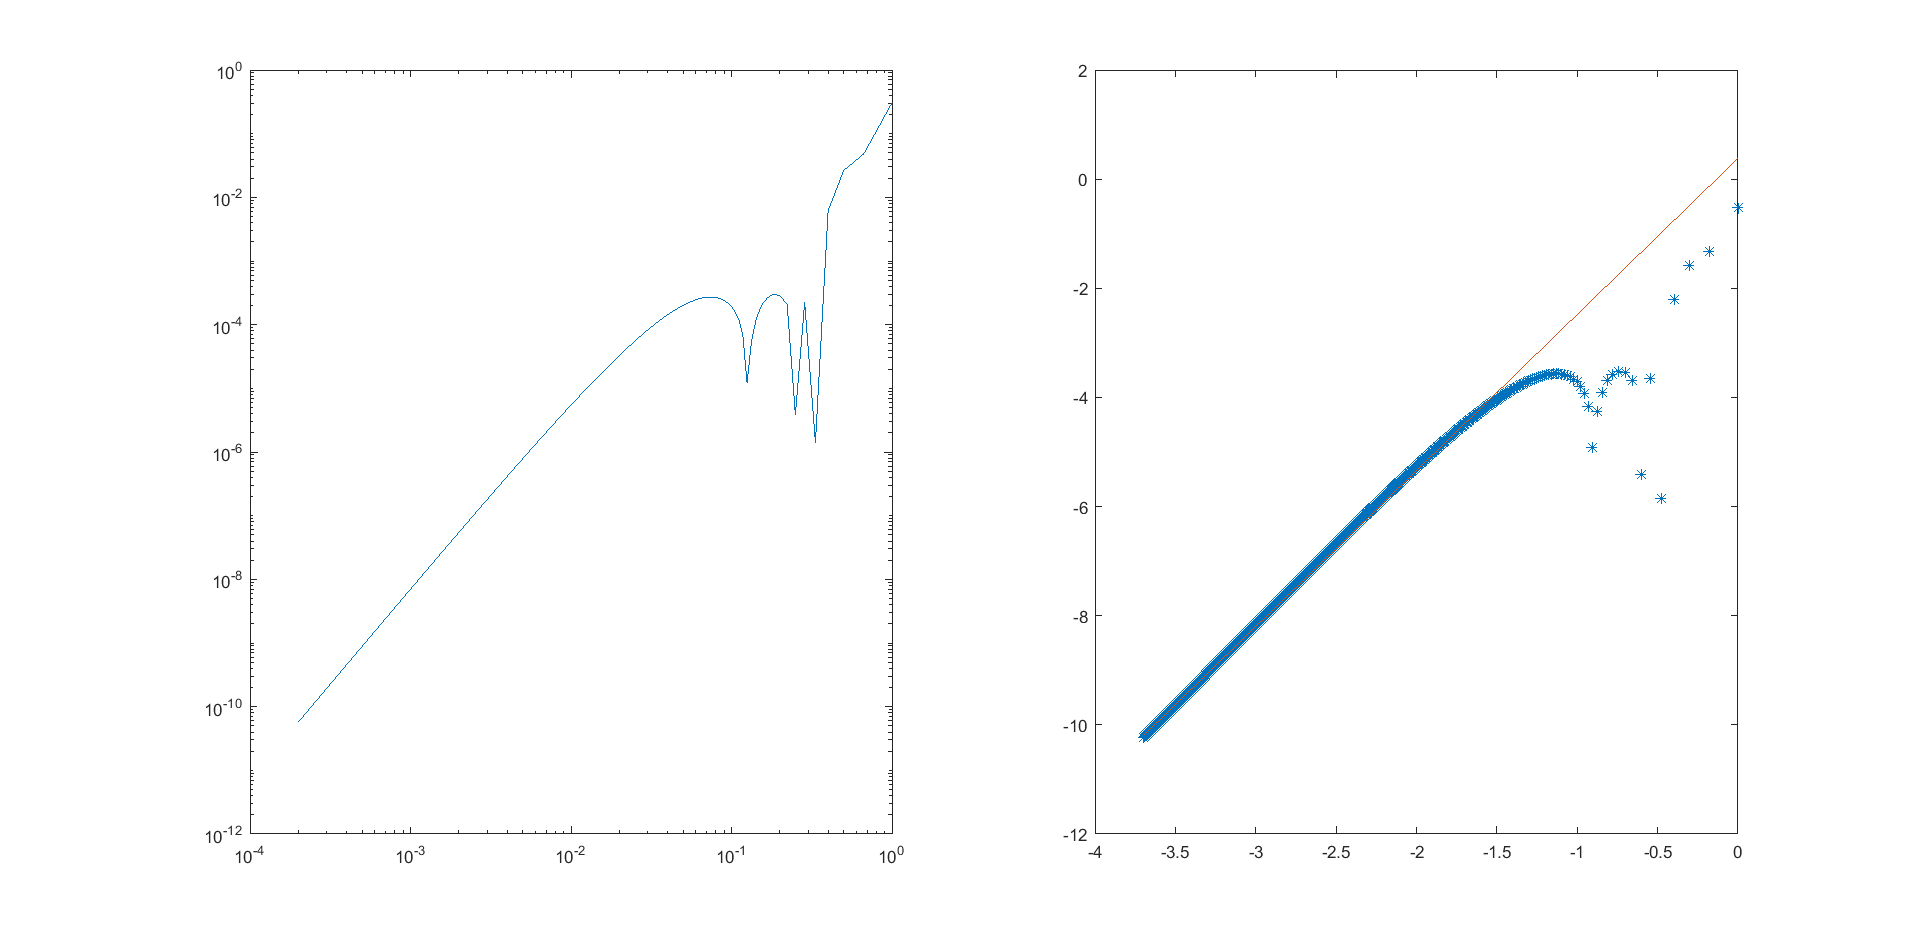
\includegraphics[scale=0.3]{3_4.png}
                        \caption{在 $x=2$ 这一点的误差随区间大小随步长变化情况}
                    \end{figure}
                    得到的拟合直线斜率为$2.86028714159494$,即所用方法的阶数为$3$。而式\ref{1}的局部截断误差为
                    $O\left(h^{5}\right)$,整体截断误差为$O\left(h^{4}\right)$,即$4$阶精度。
                    为了不影响格式的整体截断误差,起步计算的格式的精度至多只能比该格式的精度低一阶,也就是说,对于
                    本题的四阶格式,我们需要用至少三阶的Runge-Kutta格式来做起步计算。
          \end{enumerate}
\end{enumerate}


\end{document}
